\section {\textit{Netwok Time Protocol} - NTPv4}

\subsection {Introdução}

O protocolo NTP implementa diversas soluções que permitem a sincronização dos
relógios dos computadores pertencentes a uma determinada rede. O protocolo
utiliza diversas métricas, descritas nas próximas seções, a fim de determinar
quais são as fontes mais seguras e consistentes para obter a melhor
sincronização e uma maior precisão. Somadas a essas estatísticas, o NTP faz uso
de algoritmos de seleção, \textit{cluster} e combinação que garantem, por sua
vez, a determinação dos servidores mais confiáveis a partir de um número finito
de amostras provindas de tais fontes. 

\vspace{12pt}

A troca de mensagens é feita através de pacotes UDP, sendo que o protocolo
suporta tanto o IPv4 quanto o IPv6. Apesar do fato de que o protocolo UDP não
oferece garantias de entrega e correção de eventuais erros ou duplicatas, o
NTPv4 implementa mecanismos, tais como o \textit{On-Wire protocol}, capazes de
verificar a consistência dos dados contidos nos pacotes recebidos e, assim,
agir corretamente em casos de perdas ou pacotes repetidos.

\vspace{12pt}

Neste relatório, serão discutidas as características da versão 4 do NTP,
especificadas no RFC5905. Esta versão aprimora alguns aspectos da versão 3
(NTPv3) e adiciona algumas outras funcionalidades, como, por exemplo, a
descoberta dinâmica de servidores (\textit{automatic server discovery}),
sincronização rápida na inicialização da rede ou depois de falhas
(\textit{burst mode}) e uso da criptografia \textit{Public-key}.

\subsection {Características do Protocolo}

O primeiro aspecto importante do protocolo NTPv4 é a organização dos
nós de uma rede. O NTP provê 3 tipos diferentes de variantes 
e 6 modos de associação, que identificam a função de cada nó que
compõe um comunicação. As variantes NTP são, portanto:

\begin {enumerate}[i.]
  
  \item \textit{server/client}: um cliente envia pacotes a um servidor
  requisitando sincronização, que responde utilizando o endereço contido nos
  respectivos pacotes. Nesta variante, servidores fornecem sincronização aos
  clientes, mas não aceitam sincronizações vindas dos clientes. As associações
  entre os nós nesta variante são persistentes, ou seja, são criadas na
  inicialização do serviço e nunca são destruídas.
  
  \item \textit{symmetric}: neste tipo de variante, um nó se comporta tanto como
  servidor como cliente, isto é, ele recebe e envia informações de sincronização
  ao outro nó. Associações deste tipo podem ser persistentes, conforme explicado
  no item anterior, ou temporárias, isto é, podem ser criadas a partir do
  recebimento de um pacote e eliminadas após um certo intervalo ou ocorrência
  de erro. No primeiro caso, adota-se uma associação \textit{ativa}, enquanto
  que na segunda, adota-se uma \textit{passiva}.
      
  \item \textit{broadcast}: nesta variante, um servidor \textit{broadcast}
  persistente envia pacotes que podem ser recebidos por diversos clientes.
  Quando um cliente recebe um pacote deste tipo, uma associação temporária do
  tipo \textit{broadcast client} é criada e o cliente recebe sincronização até o
  fim de um intervalo ou ocorrência de um erro.
  
\end{enumerate}

O protocolo oferece ainda uma funcionalidade que permite aos clientes
descobrirem servidores disponíveis na rede para sincronização. Tal mecanismo é
chamado de \textit{Dynamic Server Discovery}, que provê dois tipos especiais de
associação: \textit{manycast server} e \textit{manycast client}. Um cliente
\textit{manycast} persistente envia pacotes para endereços de \textit{broadcast}
ou \textit{multicast} e, caso um \textit{manycast server} receba tais pacotes,
ele envia uma resposta a determinado cliente, que, por sua vez, mobiliza uma
associação temporária com o respectivo servidor. A fim de descobrir os
servidores mais próximos, os clientes enviam pacotes com TTL crescentes, até que
o número mínimo de servidores descobertos seja atingido.

\vspace{12pt}

O segundo aspecto importante é a implementação dos processos que são executados
em um sistema a fim de garantir as funcionalidades apresentadas acima. Cada nó
da rede utiliza dois processos dedicados para cada servidor que provê
sincronização, além de 3 outros dedicados para escolha dos melhores candidatos
e ajuste do relógio. A figura \ref{fig:modelo} esquematiza a relação entre tais
processos. As flechas representam trocas de dados entre processos ou algoritmos.
 
\FloatBarrier

\begin{figure}[h]
    
    \centering
    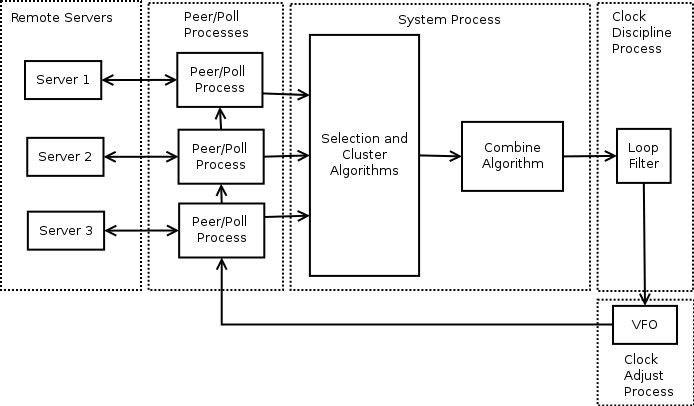
\includegraphics[scale=0.5]{image/ntp_implementation}
    \caption {Implementação dos processos executados por um nó da rede.}
    \label{fig:modelo}
\end{figure} 

\FloatBarrier

Cada componente é, portanto, responsável por uma funcionalidade específica
oferecida pelo NTP. Temos, assim:

\begin {enumerate}[i.]
  \item \textit{Remote servers}: servidores que fornecem sincronização aos nós
  da rede. Tais servidores podem pertencer à mesma rede às quais os clientes
  estão inseridos ou podem ser disponibilizados via Internet por organismos
  responsáveis por gerenciar e garantir que os relógios apresentem tempos
  consistentes. 
  
  A fim de diferenciar os diversos servidores utilizados em relação ao seu grau
  de importância e confiabilidade, o protocolo NTP atribui um nível a cada
  \textit{server}, chamado de \textit{stratum}. Tal atributo vale 1 para
  servidores primários, 2 para servidores secundários e assim sucessivamente. À
  medida que o valor de \textit{stratum} aumenta, a precisão diminui,
  dependendo do estado da rede. O valor máximo deste atributo é 15 e, portanto,
  são permitidos até 15 níveis hierárquicos. O valor 0 é reservado pelo
  protocolo para mensagens de controle e transmissão de estado entre nós. Tais
  mensagens são chamadas de pacotes \textit{Kiss-o'-Death}.
  
%   Caso \textit{stratum} de determinado servidor apresente o valor
%   16, isso significa que o cliente que está tentando obter sincronização está
%   dessincronizado com tal servidor.
  
  \item \textit{Peer/poll processes}: quando um pacote transmitido por um
  servidor chega em um nó, o \textit{peer process} é chamado. Tal processo então
  verifica se o pacote é consistente (\textit{On-Wire protocol}, proteção
  contra perdas e duplicatas) e calcula algumas estatísticas usadas pelos demais
  processos. Tais estatíticas consistem em:
  		
  		\begin{itemize}
  		  \renewcommand\labelitemi{--}
  		  \item \textit{offset} (\(\theta\)): deslocamento de tempo do
  		  relógio do servidor em relação ao relógio do sistema;
  		  \item \textit{delay} (\(\delta\)): tempo que o pacote necessita para
  		  percorrer toda a rede entre cliente e servidor;
  		  \item \textit{dispersion} (\( \epsilon \)): erro máximo inerente à medida
  		  do relógio do sistema;
  		  \item \textit {jitter} (\( \psi \)): raiz do valor quadrático médio dos
  		  \textit{offsets} mais recentes.
  		\end{itemize}
  		
	O \textit{poll process} é responsável, por sua vez, por enviar pacotes aos
	servidores a cada intervalo de \(2^\tau\) segundos. \(\tau\) varia de 4 a 17,
	resultando, assim, em intervalos de 16 segundos a 36 horas. O valor de \(\tau\)
	pode variar durante a execução, sendo modificado pelo algoritmo regulador do
	relógio, que será discutido posteriormente. 
	
	\item \textit{System process}:
\end{enumerate}

\subsection {Exemplo}

\subsection {Aplicação ao projeto \textit{Sirius}}